\section{Objective}
\label{sec:4-1}

Data Understanding and Data Preparation (Chapter~\ref{ch:data-preparation}) form one narrative: understand the data, extract insights about transactions and customers, and turn them into the strategy for building the modeling dataset -- its population, label and features. This chapter covers the first half: an overview of the data (Section~\ref{sec:4-2}), sales and seasonality (Section~\ref{sec:4-3}), why existing customers matter (Section~\ref{sec:4-4}), how often customers come back, which sets the churn definition (Section~\ref{sec:4-5}), the customer segments (Section~\ref{sec:4-6}) and how concentrated revenue is (Section~\ref{sec:4-7}). It ends with the design decisions (Section~\ref{sec:4-8}) that Chapter~\ref{ch:data-preparation} implements.

\section{Dataset Overview}
\label{sec:4-2}

The raw dataset (before any cleaning) contains:

\begin{center}
\begin{tabular}{@{}p{5cm}p{8.5cm}@{}}
    \toprule
    Metric & Value \\
    \midrule
    Transactions (rows) & 1,067,371 \\
    Invoices & 53,628 \\
    Customers & 5,942 \\
    Products & 5,305 \\
    Countries & 43 \\
    Total quantity & 10,608,492 units \\
    Total revenue (GBP) & 19,287,250.57 \\
    Date range & 2009-12-01 -- 2011-12-09 ($\approx$ 2 years) \\
    \bottomrule
\end{tabular}
\end{center}

The dataset is overwhelmingly UK-based: the \textbf{United Kingdom} accounts for 981,330 rows (91.9\%); the next largest markets are EIRE (17,866), Germany (17,624), France (14,330) and the Netherlands (5,140), each far behind the UK.

After applying the valid-purchase definition (Section~\ref{sec:5-2}), \textbf{776,577 rows (72.8\%) remain, representing 36,594 purchase occasions (invoices) of 5,852 customers} between 1 December 2009 and 9 December 2011. The rest of this chapter works on this valid-transaction subset; the per-rule data-quality breakdown is reported with the cleaning rules in Section~\ref{sec:5-2}.

\section{Monthly Sales and Seasonality}
\label{sec:4-3}

\begin{center}
\includegraphics[width=0.85\textwidth]{figures/ch6_monthly_revenue_customers.png}
\end{center}

A typical full month has about \textbf{1,040 purchasing customers} (median 965) and \textbf{revenue of about GBP 690K} (median GBP 595K), ranging from GBP 442K (Feb 2011) to GBP 1.16M (Nov 2010). Both series are clearly \textbf{seasonal}: a steady climb from late summer to a peak in \textbf{October--November} (Nov 2010: GBP 1.16M; Nov 2011: GBP 1.14M; Oct 2010 and Oct 2011: GBP 1.0M each), driven by pre-Christmas ordering, followed by a sharp fall in December (Dec 2010: GBP 565K, 884 customers) through February. The first month (Dec 2009) and the last month (Dec 2011, only 9 days of data) are partial periods.

Two consequences carry into Chapter~\ref{ch:data-preparation}. Only about 1,040 of the 5,852 customers buy in a given month, so most customers purchase infrequently and churn must be judged over a window much longer than a month. And because behavior shifts with the season, the data must be split chronologically and results read per scoring week.

\section{Existing Customers Drive Revenue}
\label{sec:4-4}

Each customer's purchase occasions are ordered in time; the first occasion is \textbf{new}, every later one is \textbf{existing}. At the customer level, over the whole period:

\begin{center}
\begin{tabular}{@{}p{3cm}p{2.3cm}p{2.3cm}p{2.6cm}p{2.3cm}@{}}
    \toprule
    Segment & Customers & Orders & Revenue (GBP) & Revenue share \\
    \midrule
    One-time & 1,618 (27.65\%) & 1,618 (4.42\%) & 555,999.97 & 3.26\% \\
    Repeat & 4,234 (72.35\%) & 34,976 (95.58\%) & 16,512,568.00 & 96.74\% \\
    \bottomrule
\end{tabular}
\end{center}

\textbf{Repeat customers} -- those with two or more purchase occasions -- are 72.3\% of the customer base but generate \textbf{95.6\% of orders and 96.7\% of revenue}. Almost all realized revenue already comes from customers who buy more than once, which is the direct business case (Chapter~\ref{ch:problem-approach}) for a retention strategy aimed at existing customers.

The same picture holds month by month. Each customer active in a month is counted once, as new in their first purchase month and existing in any later month:

\begin{center}
\includegraphics[width=0.85\textwidth]{figures/ch6_new_existing_share.png}
\end{center}

After the first months of data (Dec 2009 is 100\% new by construction), existing customers make up 80\% or more of monthly active customers from mid-2010 and 81.6--95.4\% throughout 2011, and their share of monthly revenue is higher still, in the 88--96\% range from late 2010 onward. Existing customers therefore dominate both who buys and how much is spent.

\section{Repurchase Interval and the 90-Day Horizon}
\label{sec:4-5}

Retail is a \textbf{non-contractual} setting: customers never cancel, so churn has to be inferred from a period without purchases. The gap between consecutive purchase occasions of the same customer tells how long that period should be. Note that the shares below are per \textbf{repurchase} (one gap per repeat occasion, 30,742 in total), not per customer: frequent buyers contribute more gaps, and one-time customers contribute none.

\begin{center}
\includegraphics[width=0.85\textwidth]{figures/ch6_inter_purchase_interval.png}
\end{center}

\begin{center}
\begin{tabular}{@{}p{2.3cm}p{2.3cm}p{2.3cm}p{2.3cm}p{2.3cm}@{}}
    \toprule
    Mean & Std & Median & P90 & P99 \\
    \midrule
    52.1 d & 75.9 d & 25.0 d & 136.0 d & 368.9 d \\
    \bottomrule
\end{tabular}
\end{center}

Gaps are highly right-skewed (mean 52.1 days vs.\ median 25.0 days). \textbf{54.8\% of repurchases happen within 30 days} of the previous purchase -- the largest single group, but not yet representative of repurchasing as a whole. Extending the window to \textbf{90 days covers 82.8\% of repurchases}; beyond 150 days each 30-day bin holds under 2.5\% of gaps, and the open-ended 240+ bin collects the remaining 3.7\%.

\textbf{Choosing the horizon $H$.} The prediction horizon trades off three criteria:

\begin{center}
\begin{tabular}{@{}p{1.6cm}p{5cm}p{4.6cm}@{}}
    \toprule
    $H$ (days) & Repurchases within $H$ & Training weeks after the embargoed split \\
    \midrule
    60 & 74.2\% & 37 \\
    \textbf{90} & \textbf{82.8\%} & \textbf{24} \\
    120 & 88.1\% & 10 \\
    \bottomrule
\end{tabular}
\end{center}

A shorter horizon labels as churned many customers who would in fact come back (noisier labels); a longer one detects churn later -- at odds with the goal of early identification (Section~\ref{sec:1-2}) -- and, on a two-year window, leaves far fewer labelable weeks for training once two $H$-day embargoes are subtracted (computed in Section~\ref{sec:5-6}). \textbf{$H = 90$ days} covers most repurchases while keeping 24 training weeks; moving to 120 days would add only 5 points of coverage at the cost of more than half the training weeks.

\textbf{Per repurchase vs.\ per customer.} The 82.8\% above is a share of repurchases, which frequent buyers dominate. Per customer, only \textbf{59.8\% of the 4,234 repeat customers} have an average gap under 90 days (17.8\% under 30 days, 41.9\% at 30--90 days) and 40.2\% buy more slowly; adding the one-time customers, who have no repurchase at all, explains why the churn rate at $H = 90$ is close to one half (Section~\ref{sec:5-4}) even though most repurchases happen within 90 days.

The same distribution sets the \textbf{activity threshold} $R_{\max} = $ P90 $=$ 136 days: a customer whose last purchase is older than this is treated as already lapsed and is not scored. $H$ answers \emph{how long without a purchase counts as churn}; $R_{\max}$ answers \emph{who is still worth predicting for}.

\section{Customer Segments}
\label{sec:4-6}

Customers are grouped by three behaviors measured over their \textbf{full history}: recency R (days since the last purchase, up to the day after the last transaction), frequency F (number of sales invoices) and monetary value M (sales net of returns). The thresholds come from the analysis above: $R \le 90$ days marks a customer as still active (Section~\ref{sec:4-5}), F separates one, two to three and four or more invoices, and ``high value'' is the top 10\% of M (net revenue of at least \pounds5,224). Rules are applied in order, so every customer falls into exactly one group. Customers silent for more than 90 days are first split by how long they have been away (Cooling, 91--180 days: 555; Lapsed, 181--365 days: 777; Dormant, over a year: 1,564) and then merged into one \textbf{Inactive} group:

\begin{center}
\begin{tabular}{@{}p{2.7cm}p{3.1cm}p{1.85cm}p{1.75cm}p{1.75cm}p{2cm}@{}}
    \toprule
    Segment & Rule & Customers & Customer share & Revenue share & Mean net revenue \\
    \midrule
    \textbf{Champions} & Top 10\% M, $R \le 90$ & 515 & 8.8\% & \textbf{58.1\%} & \pounds18,449 \\
    \textbf{VIP at risk} & Top 10\% M, $R > 90$ & 71 & 1.2\% & \textbf{5.2\%} & \pounds11,979 \\
    Loyal & $R \le 90$, $F \ge 4$ & 1,345 & 23.0\% & 18.9\% & \pounds2,295 \\
    Developing & $R \le 90$, $F = 2$--$3$ & 658 & 11.2\% & 3.2\% & \pounds806 \\
    One-time recent & $R \le 90$, $F = 1$ & 367 & 6.3\% & 0.8\% & \pounds369 \\
    Inactive & $R > 90$ & 2,896 & 49.5\% & 13.8\% & \pounds780 \\
    \bottomrule
\end{tabular}
\end{center}

\begin{center}
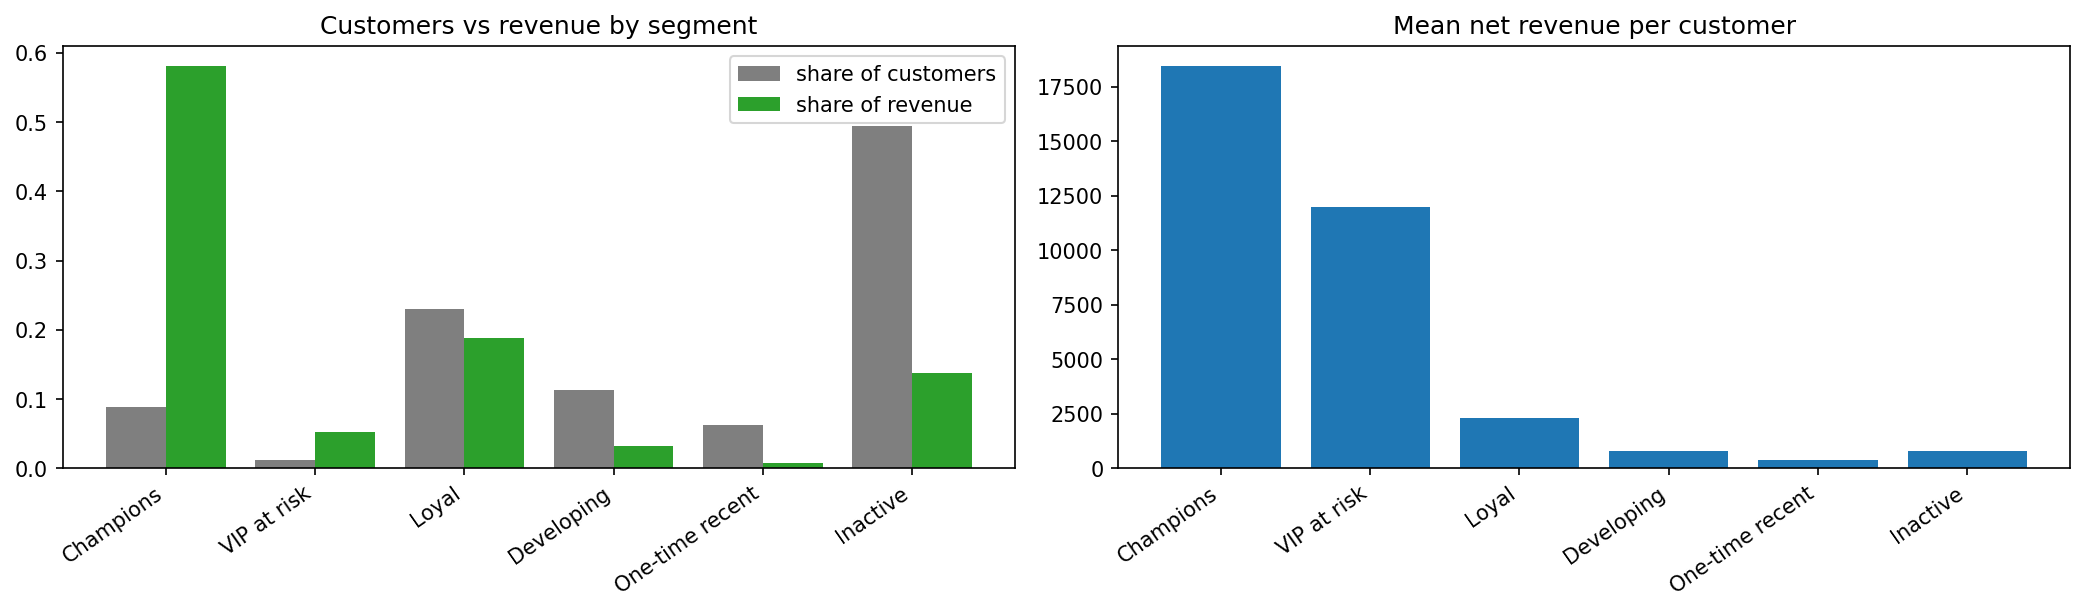
\includegraphics[width=0.95\textwidth]{figures/ch4_customer_segments.png}
\end{center}

\textbf{Two groups hold 63\% of revenue.} Champions and VIP at risk are the top 10\% of spenders: 10.0\% of customers, \textbf{63.3\% of net revenue}. VIP at risk are exactly the high-value customers who have crossed the 90-day line. At the other end, half of all customers are already inactive and bring only 13.8\% of revenue, and recent one-time buyers bring 0.8\%. The value at stake is therefore very concentrated, which is why the expected-margin option of Chapter~\ref{ch:evaluation} weighs customers by their value and why that value is capped (Section~\ref{sec:5-5}).

These segments are descriptive: they use the full history and are not model inputs. The model of Chapter~\ref{ch:modeling} only sees point-in-time features, and the score table carries the RFM quintile segments fitted on the training period (Section~\ref{sec:5-5}). The dashboard (Section~\ref{sec:8-5}) applies the same eight rules at every weekly snapshot. Source: \texttt{notebooks/02\_customer\_segments.ipynb}.

\section{Value Concentration}
\label{sec:4-7}

Revenue is concentrated in a small number of large, often wholesale, customers. Measured per customer over the full history (gross valid revenue, so the top 10\% hold 63.9\% here against 63.3\% of net revenue in Section~\ref{sec:4-6}):

\begin{center}
\begin{tabular}{@{}p{3.6cm}p{2.6cm}p{3.2cm}@{}}
    \toprule
    Customers (by revenue) & Customers & Share of revenue \\
    \midrule
    Top 1\% & 59 & 32.1\% \\
    Top 5\% & 293 & 52.0\% \\
    Top 10\% & 585 & 63.9\% \\
    Top 20\% & 1,170 & 77.2\% \\
    \bottomrule
\end{tabular}
\end{center}

\begin{center}
\includegraphics[width=0.75\textwidth]{figures/ch6_value_concentration.png}
\end{center}

The 59 customers with an average order value at or above its P99 (\pounds1,907) alone hold 19.5\% of revenue. Any value-weighted quantity, such as the expected margin of an offer (Chapter~\ref{ch:evaluation}), would therefore be dominated by a handful of wholesale-sized accounts. This motivates capping the customer value proxy V at its 99th percentile, fitted on the training period (Section~\ref{sec:5-5}), and reporting wholesale-sized customers separately in the error analysis (Section~\ref{sec:7-12}).

\section{Key Findings and Design Decisions}
\label{sec:4-8}

\begin{center}
\begin{tabular}{@{}p{7.2cm}p{7cm}@{}}
    \toprule
    Finding & Design decision (Chapter~\ref{ch:data-preparation}) \\
    \midrule
    776,577 valid rows (72.8\%) = 36,594 invoices of 5,852 customers, Dec 2009 -- Dec 2011 & Customer histories built from valid purchase occasions only (Sections~\ref{sec:5-2}--\ref{sec:5-3}) \\
    About 1,040 customers and GBP 690K revenue per month; peak in Oct--Nov, sharp drop in Dec & Chronological split with embargo; results read per scoring week (Section~\ref{sec:5-6}) \\
    Only about 1,040 of 5,852 customers buy in a given month & Weekly snapshots of all active customers, judged over a multi-month window (Section~\ref{sec:5-3}) \\
    Repeat customers: 72.3\% of customers, 95.6\% of orders, 96.7\% of revenue & Population focused on existing customers (Section~\ref{sec:5-3}) \\
    54.8\% of repurchases within 30 days, 82.8\% within 90 days; P90 gap $=$ 136 days & Label horizon $H = 90$ days (Section~\ref{sec:5-4}); activity threshold $R_{\max} = 136$ days (Section~\ref{sec:5-3}) \\
    59.8\% of repeat customers have an average gap under 90 days; one-time customers have none & A churn rate close to one half at $H = 90$ (Section~\ref{sec:5-4}) \\
    One-time customers: 27.6\% of customers, 3.3\% of revenue & Kept in the population but reported as a separate segment \\
    Revenue is concentrated: the top 1\% of customers hold 32\% of revenue, the top 10\% hold 64\% & Customer value V capped at P99 of the training period; wholesale-sized customers reported separately (Section~\ref{sec:5-5}) \\
    Six behaviour groups: Champions and VIP at risk (top 10\% of spenders) hold 63\% of revenue; half of all customers are inactive & Customer value V enters the expected-margin option (Chapter~\ref{ch:evaluation}) and is capped at P99 (Section~\ref{sec:5-5}) \\
    \bottomrule
\end{tabular}
\end{center}
